\documentclass{standalone}
\usepackage[T1]{fontenc}
\usepackage[latin2]{inputenc}
\usepackage[english]{babel}
\usepackage{tikz}
\usepackage{times}
\usetikzlibrary{calc,through,backgrounds,positioning,fit}
\usetikzlibrary{shapes,arrows,shadows,calendar}
\begin{document}

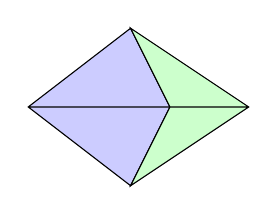
\begin{tikzpicture}
\draw[fill=white!80!blue] (0.2,0) -- (1.5,1)--(2,0)--(1.5,-1)--cycle (0.2,0)--(2,0);
\draw[fill=white!80!green] (1.5,1)--(2,0)--(1.5,-1)--(3,0)--cycle (2,0)--(3,0);

\end{tikzpicture}
\end{document}